%\documentclass[12pt,draftclsnofoot,onecolumn]{IEEEtran}
\documentclass[]{IEEEtran}
\usepackage{graphicx}
\usepackage{amsmath}
\usepackage{cite}

%\widowpenalty=10000
%\clubpenalty=10000

\begin{document}

\title{Near-Optimal Pilot Assignment in Cell-Free Massive MIMO}

\author{Raphael~M.~Guedes, José~F.~de~Rezende, and Valmir~C.~Barbosa
\thanks{This work was supported in part by Conselho Nacional de Desenvolvimento
Científico e Tecnológico (CNPq), Coordenação de Aperfeiçoamento de Pessoal de
Nível Superior (CAPES), and a BBP grant from Fundação Carlos Chagas Filho de
Amparo à Pesquisa do Estado do Rio de Janeiro (FAPERJ).
This work was also supported by MCTIC/CGI.br/São Paulo Research Foundation
(FAPESP) through projects Slicing Future Internet Infrastructures (SFI2) – grant
number 2018/23097-3, Smart 5G Core And MUltiRAn Integration (SAMURAI) – grant
number 2020/05127-2 and Programmable Future Internet for Secure Software
Architectures (PROFISSA) – grant number 2021/08211-7.
\textit{(Corresponding author: Valmir C. Barbosa.)}}
\thanks{RMG is with the State University of Rio de Janeiro, Informatics and
Computer Science Department, Rua São Francisco Xavier 524, 6th floor,
20550-900 Rio de Janeiro - RJ, Brazil. JFR and VCB are with the Federal
University of Rio de Janeiro, Systems Engineering and Computer Science Program,
Centro de Tecnologia, Sala H-319, 21941-914 Rio de Janeiro - RJ, Brazil (e-mail:
valmir@cos.ufrj.br).}}

\maketitle

\begin{abstract}
The main source of performance degradation in cell-free massive MIMO is pilot
contamination, which causes interference during uplink training and affects
channel estimation negatively. Contamination occurs when the same pilot
sequence is assigned to more than one user. This is in general inevitable, as
the number of mutually orthogonal pilot sequences corresponds to only a fraction
of the coherence interval. We introduce an algorithm for pilot assignment that
has an approximation ratio close to $\mathbf{1}$ for a plausibly large number of
orthogonal pilot sequences. It also has low computational complexity under
massive parallelism.
\end{abstract}

\begin{IEEEkeywords}
Cell-free massive MIMO,
pilot assignment,
cut problems on graphs,
approximation algorithms.
\end{IEEEkeywords}

\section{Introduction}
\label{intr}

A cell-free massive MIMO system \cite{naylm17} is characterized by a large
number $M$ of single-antenna, geographically distributed APs simultaneously
serving $K\ll M$ autonomous users via a TDD scheme. Each coherence interval,
assumed to be of duration $\tau_\mathrm{c}$ (samples), is divided into a phase
for uplink training and two others for downlink and uplink data transmission.
Training refers to the sending by each user to all APs of a
$\tau_\mathrm{p}$-sample pilot sequence (a pilot), with
$\tau_\mathrm{p}\ll\tau_\mathrm{c}$, used by each AP to estimate the channel for
subsequent downlink and uplink data transmission for that user. The APs are
capable of computationally efficient signal processing, and are moreover
connected to a CPU by a backhaul network. Two tasks the CPU handles are pilot
assignment and power allocation.

In this letter, we assume that all available pilots are orthogonal to one
another. Thus, given the number of samples $\tau_\mathrm{p}$ in a pilot,
the number of pilots is $P=\tau_\mathrm{p}$. Assigning pilots to users can be
complicated if $P<K$, since in this case at least two users must be assigned the
same pilot. This gives rise to so-called pilot contamination, whose consequence
is a reduced data rate for the users involved. The effect for user $k$ boils
down to the variance, totaled over all APs, of the interference on each AP's
estimate of the channel between itself and $k$ during uplink training
\cite{naylm17}. This total variance is given by
\begin{equation}
v_k=\sum_{k'\in U_k\setminus\{k\}}\sum_{m=1}^M\beta_{mk'},
\end{equation}
where $U_k$ is the set of users assigned the same pilot as user $k$ (itself
included) and $\beta_{mk'}$ is the large-scale fading between AP $m$ and user
$k'$.

Variance $v_k$ is fundamentally tied to the issue of pilot contamination and as
such plays a central role in minimizing its effects. This minimization can be
formulated as the problem of finding a partition of the set of users into
$P$ subsets, aiming to assign the same pilot to all users in the same subset.
The goal is to find a partition $\mathcal{P}=\{S_1,\ldots,S_P\}$ that minimizes
$\sum_{S\in\mathcal{P}}\sum_{k\in S}v_k$, where
\begin{equation}
\sum_{k\in S}v_k=
\sum_{k\in S}\sum_{k'\in S\setminus\{k\}}\sum_{m=1}^M\beta_{mk'}=
(\vert S\vert-1)\sum_{k\in S}\sum_{m=1}^M\beta_{mk}.
\label{sumSvk}
\end{equation}
This is an NP-hard optimization problem, but here we demonstrate that it can be
tackled by a greedy algorithm so that the optimum is approximated to within a
ratio that improves as the number of pilots $P$ increases.

In Section~\ref{contr}, we briefly review the relevant state of the art and
relate our contribution to it. We then recap a few system model details in
Section~\ref{smod}, following \cite{naylm17} closely. Our near-optimal algorithm
for pilot assignment is described and analyzed in Section~\ref{alg}, with
computational results and conclusion given in Section~\ref{rslt}.

\section{State of the Art and Contribution}
\label{contr}

Two baseline approaches to pilot assignment are RANDOM and GREEDY
\cite{naylm17}. More elaborate approaches from recent years include some that
use graph theory-based techniques \cite{lzja20,bdfzf21,zhlw21} and Improved
BASIC (IBASIC) \cite{qzj22}. The approaches in \cite{lzja20,bdfzf21,zhlw21} aim
to pose the problem of pilot assignment in terms of an undirected graph whose
vertices are the $K$ users. All three aim to obtain a $P$-set partition of the
vertex set, but the ones in \cite{lzja20,bdfzf21}, based respectively on vertex
coloring and on finding a maximum-weight matching on a bipartite graph, take
circuitous routes to their goals and seem oblivious to the precise definition of
partition $\mathcal{P}$ given in Section~\ref{intr}. In our view, they fail to
realize that the most direct route to finding partition $\mathcal{P}$ is to also
consider the perspective that is dual to the minimization involved in the
partition's definition. Such dual perspective is that of maximization: to find
partition $\mathcal{P}$, look for a maximum-weight $P$-cut of an edge-weighted
complete graph on $K$ vertices whose weights depend on the $\beta_{mk}$'s. A
$P$-cut is simply the set of all edges connecting vertices from different sets
of $\mathcal{P}$. The approach in \cite{zhlw21}, known as WGF, is on the other
hand firmly in line with this idea but uses edge weights that are essentially
unjustified.

In this letter, we pick up where WGF left off and contribute a new algorithm to
assign pilots to users. This algorithm looks for a maximum-weight $P$-cut on an
edge-weighted complete graph on the $K$ users. Edge weights stay true to the
principle of reflecting the variance of the interference caused by pilot
contamination during uplink training, as discussed in Section~\ref{intr}. We
call the new algorithm GEC (Greedy Edge Contraction) and prove that the total
weight of the $P$-cut it outputs accounts for a fraction of the optimal total
weight of at least $(P-1)/(P+1)$. Clearly, this lower bound on GEC's
approximation ratio approaches $1$ as $P$ increases. This is the sense in which
GEC is near-optimal. Our results in Section~\ref{rslt} confirm its superior
performance when compared to that of others.

\section{System Model Essentials}
\label{smod}

We assume APs and users to be placed in a $D\times D$ square region, at
coordinates $(x_i,y_i)$ for $i$ an AP or a user. We also assume that this region
wraps itself around the boundaries on both dimensions. For AP $m$ and user $k$,
letting $\Delta_{mk}^\mathrm{a}=\vert x_m-x_k\vert$ and likewise
$\Delta_{mk}^\mathrm{o}=\vert y_m-y_k\vert$ implies that the distance $d_{mk}$
between them is such that
\begin{equation}
d_{mk}^2=
{\textstyle\min^2}\{\Delta_{mk}^\mathrm{a},D-\Delta_{mk}^\mathrm{a}\}+
{\textstyle\min^2}\{\Delta_{mk}^\mathrm{o},D-\Delta_{mk}^\mathrm{o}\}.
\end{equation}
For $d_0,d_1$ (m) the reference distances, $f$ (MHz) the carrier frequency, and
$h_\mathrm{AP}$,$h_\mathrm{user}$ (m) the antenna heights, the path loss
$\mathrm{PL}_{mk}$ (dB) corresponding to $d_{mk}$ follows the three-slope model,
as in \cite{naylm17}. The resulting large-scale fading is
\begin{equation}
\beta_{mk}=10^{10^{-1}(\mathrm{PL}_{mk}+\sigma_\mathrm{sf}z_{mk})},
\end{equation}
where $\sigma_\mathrm{sf}$ (dB) is the shadow-fading standard deviation and
$z_{mk}\sim\mathcal{N}(0,1)$. We assume that the $z_{mk}$'s are uncorrelated
with one another and that the $\beta_{mk}$'s are available whenever needed.
Henceforth, we let $\beta_k=\sum_{m=1}^M\beta_{mk}$.

We use the SINR on the uplink to evaluate results. For user $k$, this SINR is
\begin{equation}
\mathrm{SINR}_k^\mathrm{u}=
\frac
{\eta_k\left(\sum_{m=1}^M\gamma_{mk}\right)^2}
{\sum_{k'\in U_k\setminus\{k\}}
\eta_{k'}a_{kk'}+\sum_{k'=1}^K\eta_{k'}b_{kk'}+c_k},
\label{sinr}
\end{equation}
where
\begin{equation}
\gamma_{mk}=\frac
{\tau_\mathrm{p}\rho_\mathrm{p}\beta_{mk}^2}
{\tau_\mathrm{p}\rho_\mathrm{p}\sum_{k'\in U_k\setminus\{k\}}\beta_{mk'}+1},
\end{equation}
\begin{equation}
a_{kk'}=\left(\sum_{m=1}^M \gamma_{mk}\frac{\beta_{mk'}}{\beta_{mk}}\right)^2,
\end{equation}
$b_{kk'}=\sum_{m=1}^M\gamma_{mk}\beta_{mk'}$, and
$c_k=\rho_\mathrm{u}^{-1}\sum_{m=1}^M\gamma_{mk}$.
In the expressions for $\gamma_{mk}$ and $c_k$, $\rho_\mathrm{p}$ and
$\rho_\mathrm{u}$ are the normalized uplink SNR for training and for data
transmission, respectively. The resulting throughput for user $k$ is
\begin{equation}
R_k^\mathrm{u}=
\frac{B}{2}
\left(1-\frac{\tau_\mathrm{p}}{\tau_\mathrm{c}}\right)
\log_2(1+\mathrm{SINR}_k^\mathrm{u}),
\label{rate}
\end{equation}
where $B$ (Hz) is the channel bandwidth.

The $\eta_k$'s appearing in Eq.~(\ref{sinr}) are power control coefficients.
The determination of these coefficients is commonly referred to as power
allocation and depends on pilots having already been assigned to users. As
customary, in order to ensure fairness toward all users we express power
allocation as the max-min problem, on variables $t$ and $\eta_1,\ldots,\eta_K$,
given by
\begin{align}
\text{maximize } &t \\
\text{subject to }
&t\le\mathrm{SINR}_k^\mathrm{u}, &k=1,\ldots,K;
\label{cvx1} \\
&0\le\eta_k\le 1, &k=1,\ldots,K.
\label{cvx2}
\end{align}
This is a quasilinear problem, so we do bisection on variable $t$ to solve it,
tackling only the linear feasibility program given by Eqs.~(\ref{cvx1})
and~(\ref{cvx2}) for each fixed value of $t$. The resulting
$\mathrm{SINR}_k^\mathrm{u}$ is necessarily the same for every user $k$. Thus,
whenever referring to these SINR values or the corresponding throughputs, we
henceforth use simply $\mathrm{SINR^u}$ and $R^\mathrm{u}$, respectively.

The $\eta_k$'s are also used by GREEDY, since its operation depends on the
$\mathrm{SINR}_k^\mathrm{u}$ values. To compute these values, we follow the
common choice of $\eta_k=1$ for every user $k$ \cite{naylm17}.

\section{Near-Optimal Pilot Assignment}
\label{alg}

GEC does pilot assignment to users by solving the MAX~$P$-CUT problem on an
edge-weighted complete graph, denoted by $G_K$, having a vertex set that
corresponds to the set of users. MAX~$P$-CUT asks that the vertex set of $G_K$
be partitioned into $P$ sets in such a way that the sum of the weights of all
inter-set edges is maximized, or equivalently the sum over all intra-set edges
is minimized.

The idea is for each of these $P$ sets to correspond to a set of users to which
the same pilot is assigned. It is therefore crucial that weights be selected in
a way that relates directly and clearly to the potential for pilot contamination
between the users in question. In line with our reasoning in Section~\ref{intr},
we quantify some user $k$'s contribution to the pilot-contamination effect on
each of the users it shares the pilot with as $\beta_k$. Thus, the weight of the
edge interconnecting vertices $i$ and $j$ in $G_K$, denoted by $w_{ij}$, is
\begin{equation}
w_{ij}=\beta_k+\beta_{k'},
\label{weight-init}
\end{equation}
assuming that vertex $i$ corresponds to user $k$ and vertex $j$ to user $k'$ (or
$i$ to $k'$, $j$ to $k$).

MAX~2-CUT (or simply MAX~CUT) is one of the classic NP-hard problems, so the
trivially more general MAX~$P$-CUT is NP-hard as well. We approach its solution
by generalizing the algorithm for MAX~CUT given in \cite{kkbh08}. The resulting
GEC runs for $P-K$ iterations, each consisting in the contraction of an edge,
say $(i^*,j^*)$, thus joining vertices $i^*$ and $j^*$ into a single new vertex,
say $\ell$, and moreover connecting to $\ell$ every vertex previously connected
to $i^*$ or $j^*$.

These iterations result in a sequence of graphs that, like the initial $G_K$,
are also edge-weighted complete graphs. Unlike $G_K$, however, vertices in these
graphs are no longer necessarily identified with single users, but generally
with non-singleton sets of users as well. The last graph in the sequence,
denoted by $G_P$, has $P$ vertices, one for each pilot.

The general formula for the weight $w_{ij}$ between vertices $i$ and $j$, valid
for all graphs in the sequence, is
\begin{align}
w_{ij}
&= \sum_{k\in S_i}\sum_{k'\in S_j}\beta_k+
\sum_{k\in S_j}\sum_{k'\in S_i}\beta_k \\
&= n_j\sum_{k\in S_i}\beta_k+
n_i\sum_{k\in S_j}\beta_k,
\label{weight-general}
\end{align}
where $S_i$ is the set of users to which vertex $i$ corresponds and $n_i$ is its
size. This expression generalizes the one in Eq.~(\ref{weight-init}), which
refers to an edge in $G_K$ with $S_i=\{k\}$ and $S_j=\{k'\}$ (or vice versa). In
order for the formula in Eq.~(\ref{weight-general}) to remain valid as vertices
$i^*$ and $j^*$ are joined to form vertex $\ell$, it suffices that each edge
$(i,\ell)$ such that $i\neq i^*,j^*$ be given weight
$w_{i\ell}=w_{ii^*}+w_{ij^*}$, that is, the sum of the weights of the two edges
that used to connect $i$ to $i^*$ and $j^*$ before the contraction of edge
$(i^*,j^*)$. Note also that summing up the edge weights of all pairs of distinct
users in $S_i$ yields
\begin{equation}
\sum_{k\in S_i}\sum_{\genfrac{}{}{0pt}{}{k'\in S_i}{k'\neq k}}\beta_k=
(n_i-1)\sum_{k\in S_i}\beta_k,
\label{contamination}
\end{equation}
which is a straightforward rewrite of Eq.~(\ref{sumSvk}). The sum of this
quantity over all vertices (every $i$) is what is targeted for minimization as
the solution to MAX~$P$-CUT is approximated by GEC. The heart of GEC at each
iteration is therefore to select for contraction the edge of least weight. GEC
is summarized as the following steps.
\begin{enumerate}
\item{}
$G\leftarrow G_K$;
\item{}
$n\leftarrow K$;
\item{}\label{jump}
If $n=P$, go to Step~\ref{laststep};
\item{}\label{firstinloop}
Let $(i^*,j^*)$ be a minimum-weight edge of $G$;
\item{}
$S\leftarrow S_{i^*}\cup S_{j^*}$;
\item{}\label{cost2a}
For each $i\neq i^*,j^*$, do $w^{(i)}\leftarrow w_{ii^*}+w_{ij^*}$;
\item{}
Contract edge $(i^*,j^*)$ by joining vertices $i^*$ and $j^*$ into a new
vertex $\ell$;
\item{}
$S_\ell\leftarrow S$;
\item{}\label{cost2b}
For each $i\neq\ell$, do $w_{i\ell}\leftarrow w^{(i)}$;
\item{}
$n\leftarrow n-1$;
\item{}\label{lastinloop}
If $n>P$, go to Step \ref{firstinloop};
\item{}\label{laststep}
$G_P\leftarrow G$;
\end{enumerate}

An extension of the analysis in \cite{kkbh08} reveals that
\begin{equation}
W^\mathrm{obt}\ge\frac{P-1}{P+1}\,W^\mathrm{opt},
\end{equation}
where $W^\mathrm{obt}$ is the total weight of the edges of $G_P$ (i.e., the
total weight of the obtained $P$-cut of $G_K$) and $W^\mathrm{opt}$ is its
optimal value. To see that this holds, let $W_K$ be the total weight of the
edges of $G_K$ and then use Lemma~1 from \cite{kkbh08}, which is valid for
MAX~$P$-CUT as much as it is for MAX~CUT. It states that
\begin{equation}
W^\mathrm{ctr}\le\frac{2(K-P)}{(K-1)(P+1)}\,W_K,
\label{lemma1}
\end{equation}
where $W^\mathrm{ctr}$ is the total weight of the $P-K$ edges contracted during
the iterations. Using Eq.~(\ref{lemma1}) and the fact that
$W_K\ge W^\mathrm{opt}$, we obtain
\begin{align}
W^\mathrm{obt} &= W_K-W^\mathrm{ctr} \\
&\ge W_K-\frac{2(K-P)}{(K-1)(P+1)}\,W_K \\
&\ge \frac{(K-1)(P+1)-2(K-P+P-1)}{(K-1)(P+1)}\,W_K \\
&\ge \frac{(K-1)(P-1)}{(K-1)(P+1)}\,W^\mathrm{opt} \\
&= \frac{P-1}{P+1}\,W^\mathrm{opt}. 
\end{align}
This means that GEC is capable of approximating the optimal $P$-cut of $G_K$ so
long as the number $P$ of pilots is sufficiently large. For example, we get
$W^\mathrm{obt}\ge 0.92\,W^\mathrm{opt}$ for $P=25$,
$W^\mathrm{obt}\ge 0.96\,W^\mathrm{opt}$ for $P=50$,
$W^\mathrm{obt}\ge 0.98\,W^\mathrm{opt}$ for $P=100$. Thus, insofar as the
summation in Eq.~(\ref{contamination}) is, as discussed in Section~\ref{intr},
a good model of how much the pilot shared by all users in $S_i$ gets
contaminated, assigning pilots to users with the aid of GEC is poised to yield
good results in practice if a relatively high number of pilots can be used.

As for GEC's computational complexity, note that its costliest step is
Step~\ref{firstinloop}, which requires $O(K^2\log K)$ time for sorting $O(K^2)$
weights, followed by Steps~\ref{cost2a} and~\ref{cost2b}, each running in $O(K)$
time. Considering that Steps~\ref{firstinloop}--\ref{lastinloop} repeat
$K-P$ times, the overall time required by GEC on a sequential
device is $O(K^3\log K)$. However, so long as ASICs can be designed
to provide the necessary massive parallelism, the time requirement of
Step~\ref{firstinloop} can be lowered to $O(\log^2K)$ (see, e.g., \cite{abss15}
and references therein). Likewise, Steps~\ref{cost2a} and~\ref{cost2b} can much
more easily be sped up to run in $O(1)$ time. The overall time required by GEC
can therefore be reduced to $O(K\log^2K)$. This remains unaltered if we add the
time for calculating the $\beta_k$'s, whenever the $\beta_{mk}$'s change , prior
to running GEC. Once again assuming the necessary massive parallelism, this can
be achieved in $O(\log M)$ time, which gets reduced to $O(\log K)$ for $M=aK$
with $a$ a constant. Since by assumption we have $K\ll M$, for consistency we
require only that $a>1$ (we use $a=4$ for our computational results).

\section{Computational Results and Conclusion}
\label{rslt}

We use the parameter values given in Table~\ref{tab1}, where the value of
$\rho_\mathrm{p},\rho_\mathrm{u}$ is for the channel bandwidth $B$ in the table,
a transmit power of $0.1$~W, a temperature of $290$~K, and a noise figure of
$9$~dB. Each value of $\tau_\mathrm{c}$ is compatible either with mobile users
at highway speeds ($\tau_\mathrm{c}=750$; see Table~2.1 in \cite{mlyn16}) or
with users at urban-road speeds ($\tau_\mathrm{c}=1000,1250$, extending that
same table for a speed of at most $18$ m/s). We use $M=400$ and $K=100$
throughout.

\begin{table}[t] 
\caption{System Model Parameters}
\label{tab1}
\centering
\begin{tabular}{ccc}
\hline
$D=10^3$~m & $d_0=10$~m & $d_1=50$~m \\
$f=1.9\times 10^3$~MHz & $h_\mathrm{AP}=15$~m & $h_\mathrm{user}=1.65$~m \\
$\sigma_\mathrm{sf}=8$~dB & $\rho_\mathrm{p}=1.57\times 10^{11}$ & $\rho_\mathrm{u}=1.57\times 10^{11}$ \\
$B=2\times 10^7$~Hz & $\tau_\mathrm{c}=750,1000,1250$ & $P=\tau_\mathrm{p}\le 100$ \\
\hline
\end{tabular}

\end{table}

For each value of $P\le K$, every result we report is an average over $10^4$
random trials, each beginning with the independent sampling of coordinates for
all $M$ APs and all $K$ users, and of values for all $z_{mk}$'s. The resulting
instance of the pilot-assignment problem is then submitted to GEC and five other
algorithms: an Improved WGF (IWGF) that uses the edge weights in
Eq.~(\ref{weight-init}), the original WGF, IBASIC, GREEDY, and RANDOM. Our
results are given in Figures~\ref{figsinr} and~\ref{figrate}, respectively for
$\mathrm{SINR^u}$ and $S^\mathrm{u}$ as functions of $P$. To avoid cluttering,
we omit confidence intervals from the figures but inform their bounds in the
figures' captions.

\begin{figure}[t]
\centering
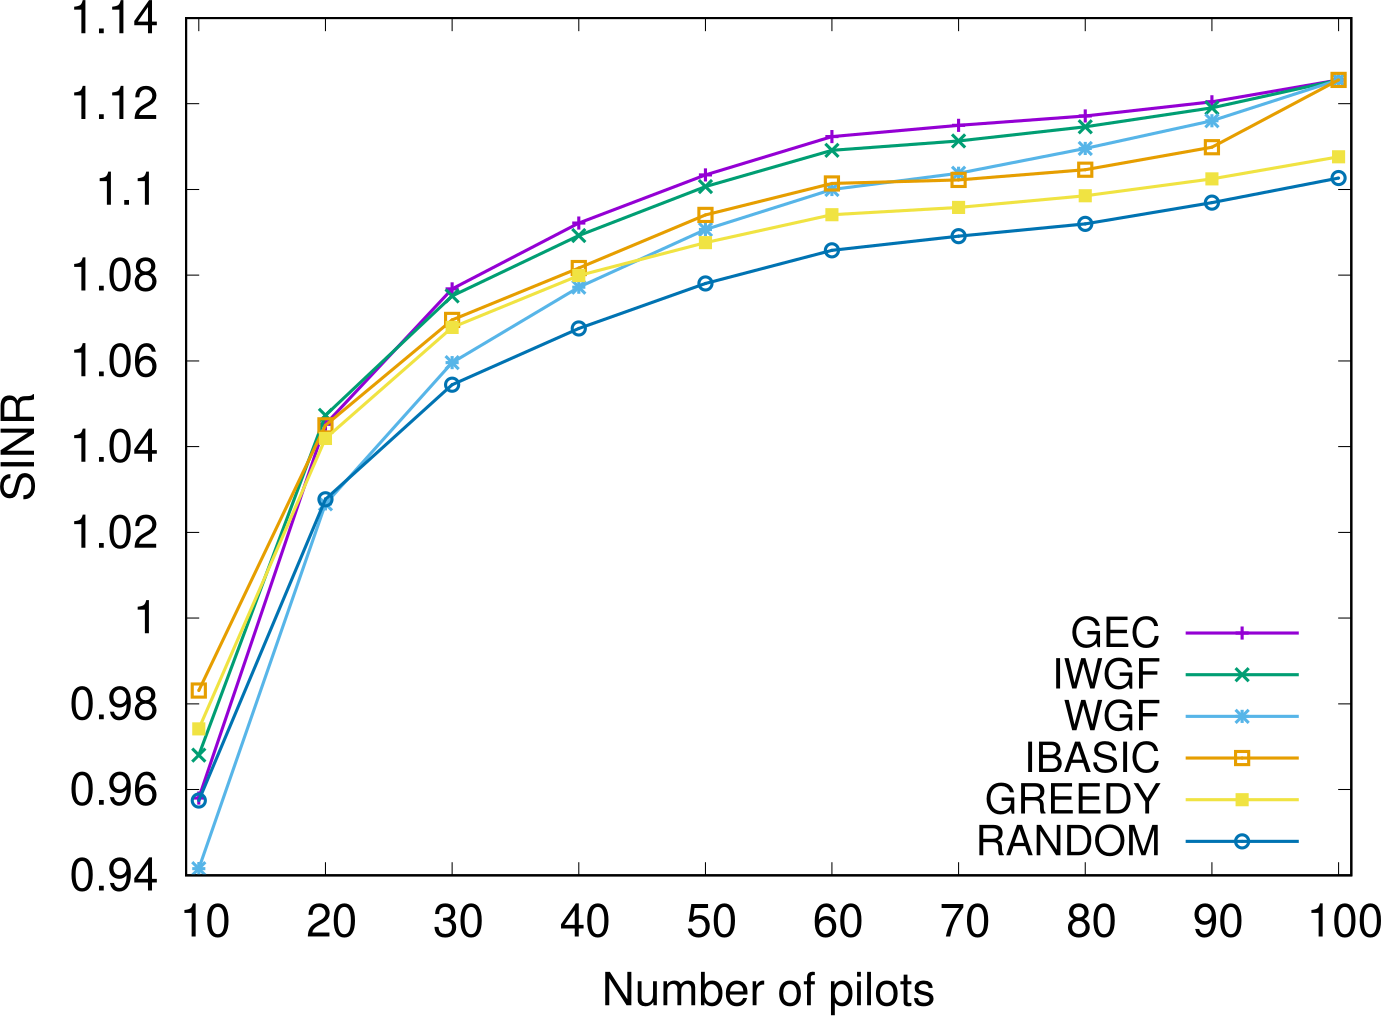
\includegraphics[scale=0.6915]{sinr.png}
\caption{$\mathrm{SINR}^\mathrm{u}$ vs.\ number of pilots $P$.
Confidence-interval bounds at the $95\%$ level are about $\pm 0.4\%$ of the
average and occur for WGF at $P=10$.}
\label{figsinr}
\end{figure}

\begin{figure}[t]
\centering
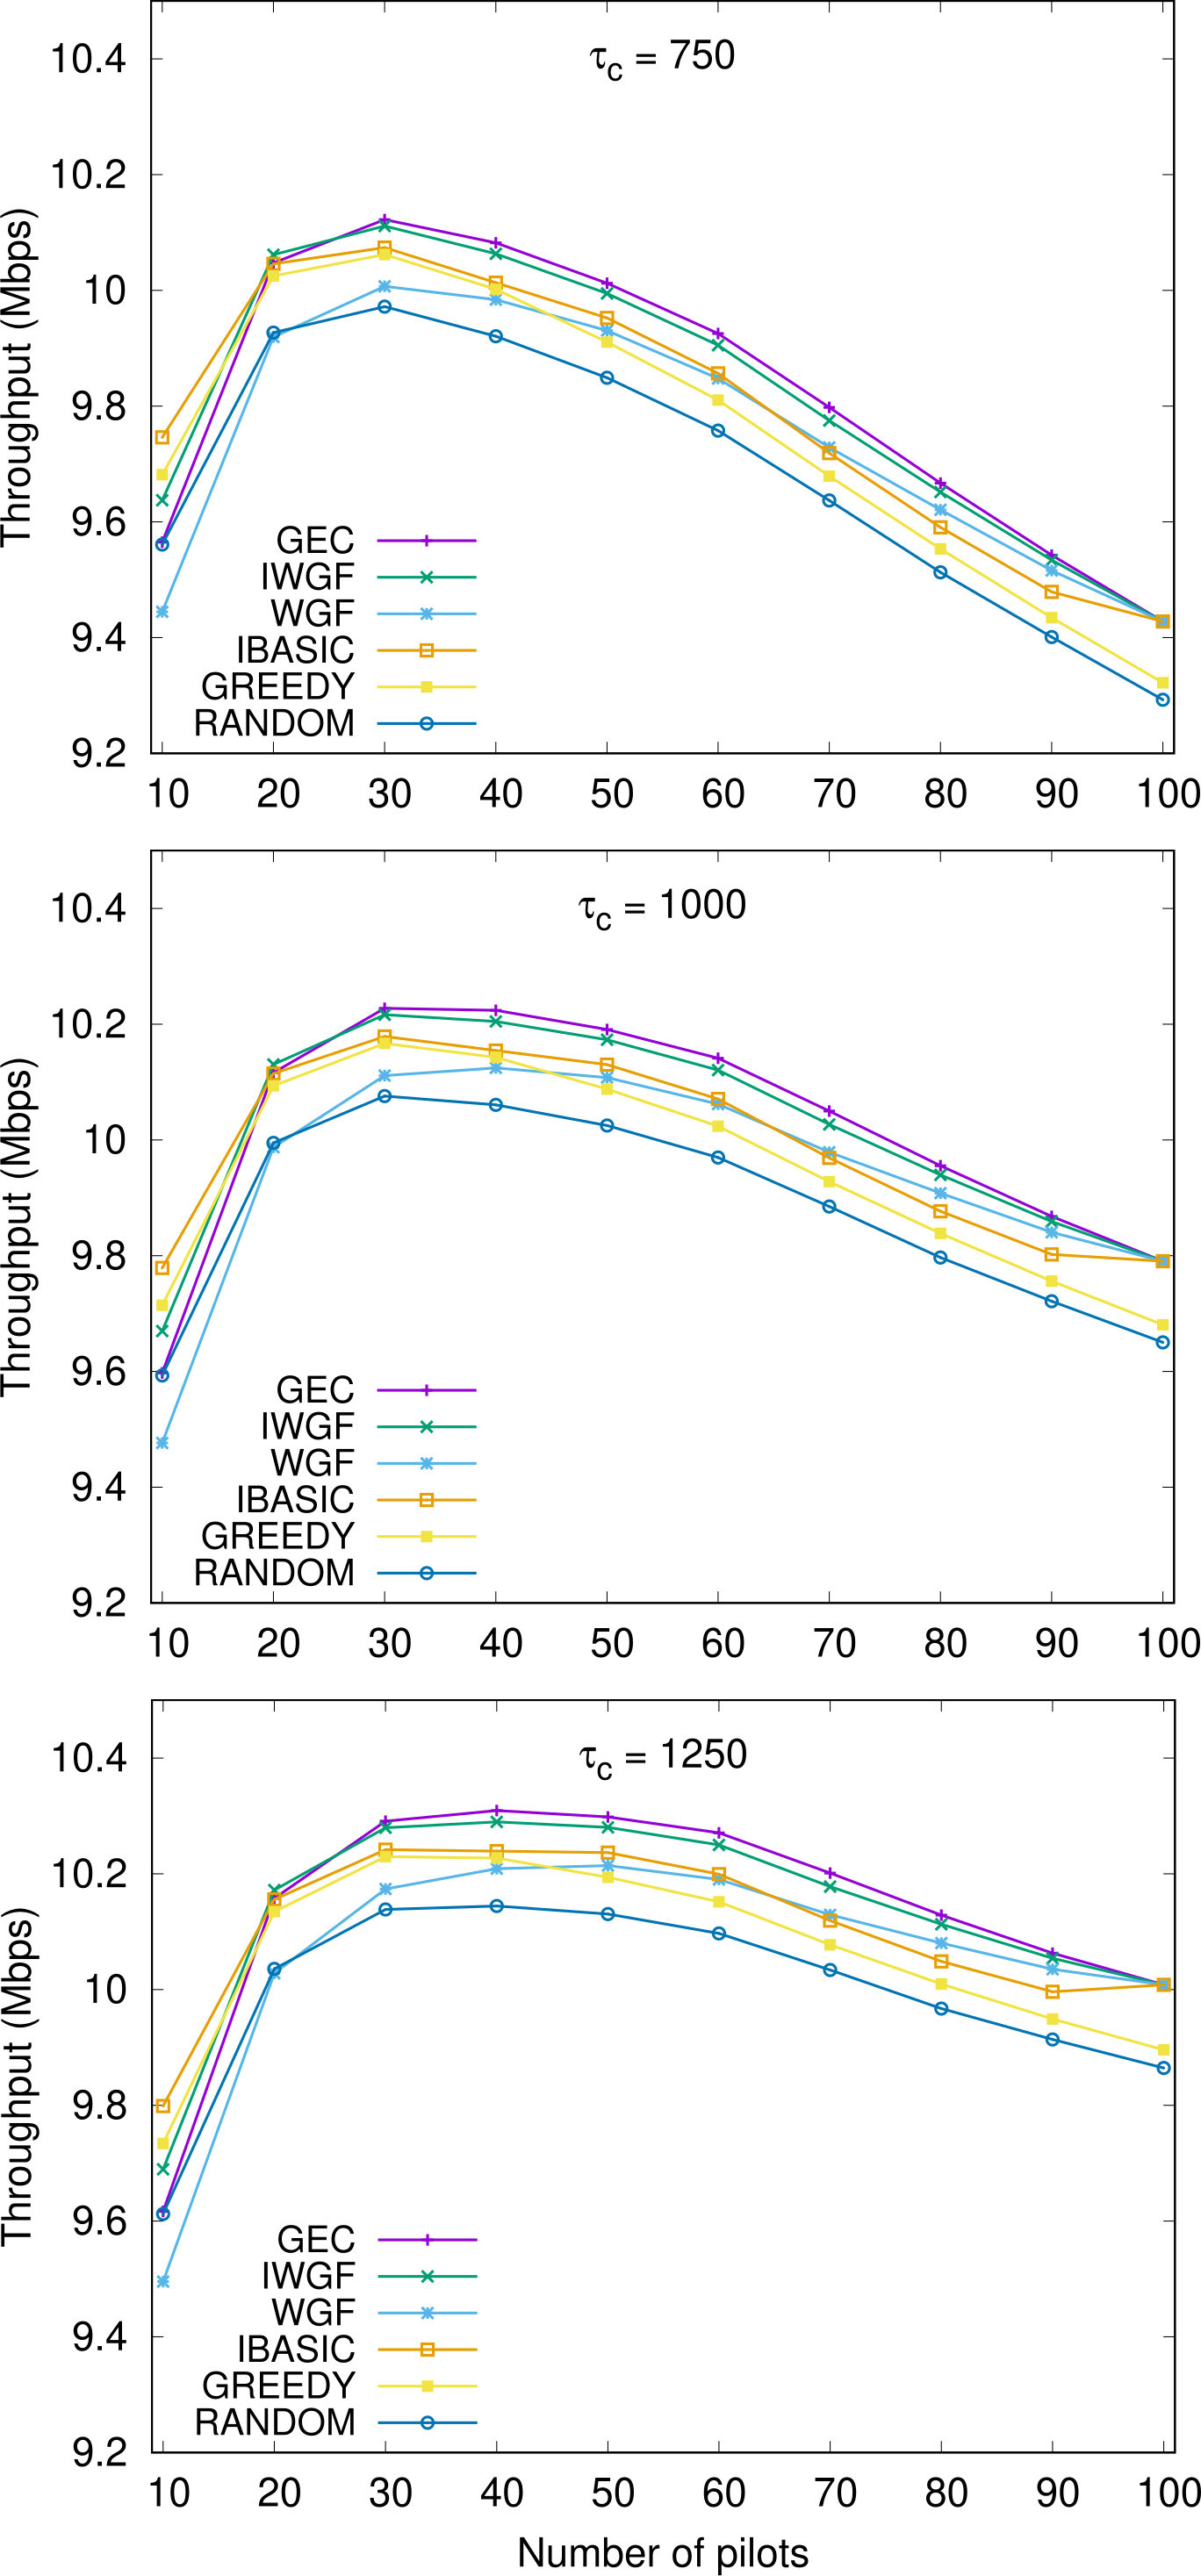
\includegraphics[scale=0.6915]{rate.png}
\caption{Throughput $R^\mathrm{u}$ vs.\ number of pilots $P$.
Confidence-interval bounds at the $95\%$ level are about $\pm 0.3\%$ of the
average and occur for WGF at $P=10$. This percentage varies with
$\tau_\mathrm{c}$ in the order of $10^{-11}$.}
\label{figrate}
\end{figure}

All plots suggest the superiority of GEC beginning at $P\approx 25$, followed
by IWGF, then variously by IBASIC, GREEDY, or WGF, though GREEDY is outperformed
by IBASIC and WGF beginning at $P\approx 45$. Excluding GREEDY and RANDOM, all
methods perform equally for $P=K$, indicating that they correctly avoid pilot
contamination altogether whenever possible. In the case of GEC, this is easily
seen by noting that the jump in Step~\ref{jump} is taken if $P=K$. In conformity
with Eq.~(\ref{rate}), throughput is seen to increase with $\tau_\mathrm{c}$ for
fixed $P$, but for fixed $\tau_\mathrm{c}$ decreases after peaking as $P$
continues to grow. This decrease is often referred to as a diminishing of the
channel's spectral efficiency, which is given by $2B^{-1}R^\mathrm{u}$.

In conclusion, we attribute the superiority of both GEC and IWGF to their
formulation as a MAX~$P$-CUT problem with edge weights that reflect the
fundamental quantity underlying the rise of pilot contamination when a pilot is
assigned to more than one user. The superiority of GEC over IWGF is a
consequence of GEC's near-optimal nature, quantified as an approximation ratio
that approaches $1$ for any reasonably large number of pilots. Additionally, the
importance of using appropriate edge weights becomes strikingly evident as we
compare IWGF with WGF, as the weights used by the latter make little sense in
regard to minimizing pilot contamination.

\bibliography{cellfree-abbrev}
\bibliographystyle{IEEEtran}

\end{document}

